

\subsection{Replay Scheduling in Continual Learning}\label{paperC:sec:replay_scheduling_in_continual_learning}

In this section, we describe our setup for enabling the scheduling for selecting replay memories at different time steps. We define a replay schedule as a sequence $S = (\va_1, \dots, \va_{T-1})$, where the task proportions $\va_i = (a_1, \dots, a_{T-1})$ for $1 \leq i \leq T-1$ are used for determining how many samples from seen tasks with which to fill the replay memory at task $i$. We construct an action space with a discrete number of choices of task proportions that can be selected at each task: At task $t$, we have $t-1$ historical tasks that we can choose samples from. We create $t-1$ bins $\vb_t = [b_1, \dots, b_{t-1}]$ and sample a task index for each bin $b_i \in \{1, \dots, t-1\}$. The bins are treated as interchangeable and we only keep the unique choices. For example, at task 3, we have seen task 1 and 2, so the unique choices of vectors are $[1,1], [1,2], [2,2]$, where $[1,1]$ indicates that all memory samples are from task 1, $[1,2]$ indicates that half memory is from task 1 and the other half are from task etc. We count the number of occurrences of each task index in $\vb_t$ and divide by $t-1$ to obtain the task proportion, i.e., $\va_t = \texttt{bincount}(\vb_t) / (t-1)$. We round the number of replay samples from task $i$, i.e., $a_i \cdot M$, up or down accordingly to keep the memory size $M$ fixed when filling the memory. From this specification, we can build a tree of different replay schedules to evaluate with the network. We outline the steps for creating the action space in Algorithm \ref{paperC:alg:action_space_discretization} (see Appendix \ref{paperC:app:rs_mcts_algorithm}). 


\begin{wrapfigure}{r}{0.64\textwidth}
	\centering
	\setlength{\figwidth}{.64\textwidth}
	\setlength{\figheight}{.27\textheight}
	\vspace{-3mm}
	\definecolor{color0}{rgb}{0.945098039215686,0.435294117647059,0.125490196078431}
\definecolor{color1}{rgb}{0.843137254901961,0.6,0.133333333333333}
\definecolor{color2}{rgb}{0.250980392156863,0.337254901960784,0.631372549019608}
\definecolor{color3}{rgb}{1,0.498039215686275,0}
\definecolor{color4}{rgb}{0.94509803921,0.23529411764,0.12549019607}
\definecolor{color5}{rgb}{0.94509803921,0.23529411764,0.12549019607}

\resizebox{0.95\textwidth}{!}{
\begin{tikzpicture}[
    roundnode/.style={circle, draw=color3, text=color3, very thick, minimum size=7mm},
    squarednode/.style={rectangle, draw=black, fill=white, text=black, very thick, minimum size=7mm, align=center, rounded corners},
    %tasknode/.style={rectangle, draw=blue!50, fill=blue!10, text=black, very thick, minimum size=7mm, align=center, depth=2cm, rounded corners},
    %task/.style={rectangle, rounded corners, thick,inner sep=3pt},
    ]
    %%% Task 1 level
    \draw[draw=blue!50, fill=blue!10, very thick, rounded corners] (0,0) rectangle (16,-2);
    \node[squarednode] (dataset1) at (1.,-1) { \textbf{Task 1} \\ 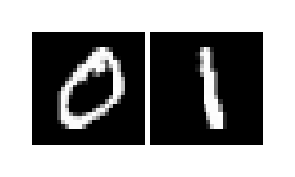
\includegraphics[width=0.08\textwidth]{PaperC/figures/mcts_tikz/dataset_two_images/dataset1.eps}};
    \node[squarednode] (v1) at (9,-1) {\large $\emptyset$};
    
    %%% Task 2 level
    \draw[draw=red!50, fill=red!10, very thick, rounded corners] (0,-2) rectangle (16,-4);
    
    \node[squarednode] (dataset2) at (1.,-3) { \textbf{Task 2} \\ 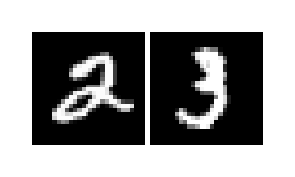
\includegraphics[width=0.08\textwidth]{PaperC/figures/mcts_tikz/dataset_two_images/dataset2.eps}};
    \node[squarednode, text=color3] (v2) at (9,-3) {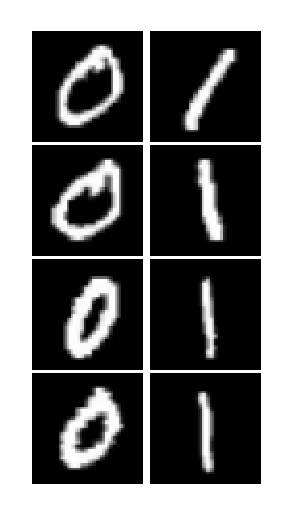
\includegraphics[width=0.045\textwidth]{PaperC/figures/mcts_tikz/vertical_rs/task1_only.eps}};
    \draw[<-] (v2) -- (v1);
    
    %%% Task 3 level
    \draw[draw=color3!50, fill=color3!10, very thick, rounded corners] (0,-4) rectangle (16,-6);
    \node[squarednode] (dataset3) at (1.,-5) { \textbf{Task 3} \\ 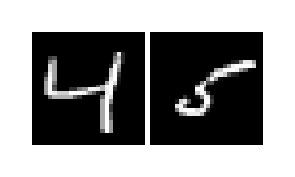
\includegraphics[width=0.08\textwidth]{PaperC/figures/mcts_tikz/dataset_two_images/dataset3.eps}};
    \node[squarednode, text=color3] (v3_beg) at (5,-5) {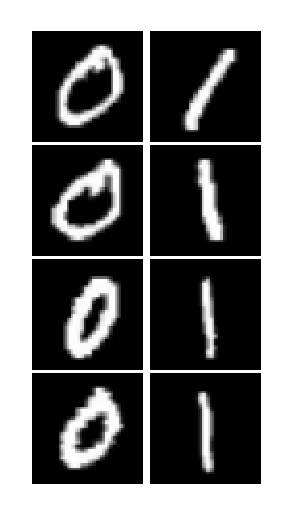
\includegraphics[width=0.045\textwidth]{PaperC/figures/mcts_tikz/vertical_rs/task1_only.eps}};
    \draw[<-, blue, very thick] (v3_beg) -- (v2);
    
    \node[squarednode, text=color3] (v3_mid) at (9,-5) {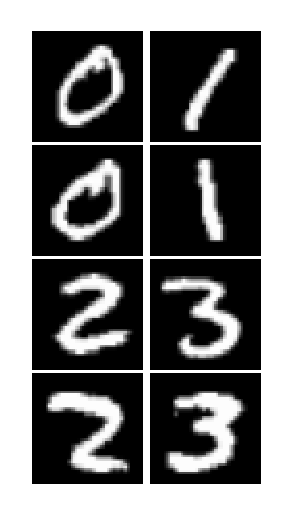
\includegraphics[width=0.045\textwidth]{PaperC/figures/mcts_tikz/vertical_rs/equal_task3.eps}};
    \draw[<-, red, very thick] (v3_mid) -- (v2);
    
    \node[squarednode, text=color3] (v3_end) at (13,-5) {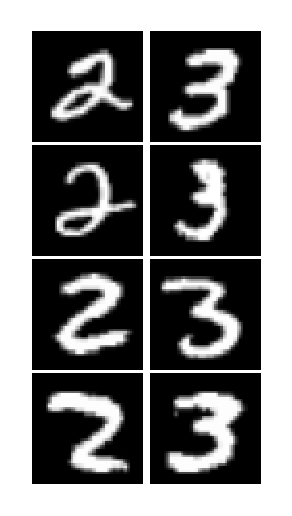
\includegraphics[width=0.045\textwidth]{PaperC/figures/mcts_tikz/vertical_rs/task2_only.eps}};
    \draw[<-, purple, very thick] (v3_end) -- (v2);
    
    %%% Task 4 level
    \draw[draw=magenta!50, fill=magenta!10, very thick, rounded corners] (0,-6) rectangle (16,-8);
    
    \node[squarednode] (dataset4) at (1.,-7) { \textbf{Task 4} \\ 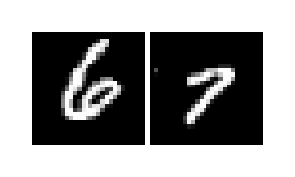
\includegraphics[width=0.08\textwidth]{PaperC/figures/mcts_tikz/dataset_two_images/dataset4.eps}};
    
    \node[squarednode, text=color3] (v41_beg) at (4,-7) {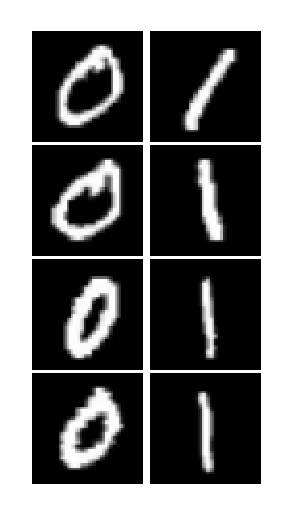
\includegraphics[width=0.045\textwidth]{PaperC/figures/mcts_tikz/vertical_rs/task1_only.eps}};
    \draw[<-, blue, very thick] (v41_beg) -- (v3_beg);
    %\draw[<-] (v4_beg) -- (v3_mid);
    %\draw[<-] (v4_beg) -- (v3_end);
    
    \node[] (v41_dots) at (5,-7) {\large $\cdots$};
    %\draw[<-] (v4_dots1) -- (v3_beg);%\draw[<-, dashed] (v4_dots1) -- (v3_beg);
    %\draw[<-] (v4_dots1) -- (v3_mid);
    %\draw[<-] (v4_dots1) -- (v3_end);
    
    \node[squarednode, text=color3] (v41_end) at (6,-7) {\includegraphics[width=0.045\textwidth]{PaperC/figures/mcts_tikz/vertical_rs/task3_only.eps}};
    \draw[<-] (v41_end) -- (v3_beg);
    
    \node[squarednode, text=color3] (v42_beg) at (7.1,-7) {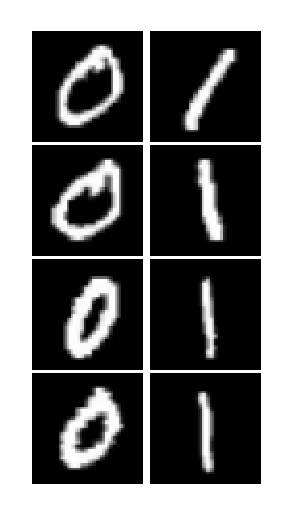
\includegraphics[width=0.045\textwidth]{PaperC/figures/mcts_tikz/vertical_rs/task1_only.eps}};
    \draw[<-] (v42_beg) -- (v3_mid);
    
    \node[] (v42_dots1) at (8,-7) {\large $\cdots$};
    
    \node[squarednode, text=color3] (v42_mid) at (9,-7) {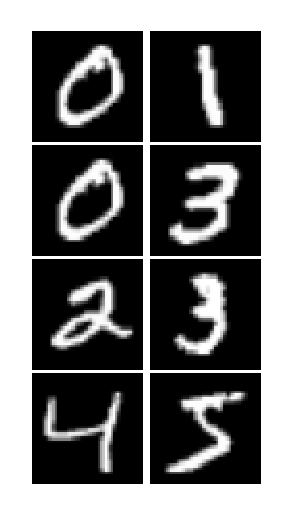
\includegraphics[width=0.045\textwidth]{PaperC/figures/mcts_tikz/vertical_rs/equal_task4.eps}};
    \draw[<-, red, very thick] (v42_mid) -- (v3_mid);
    
    \node[] (v42_dots2) at (10,-7) {\large $\cdots$};
    
    \node[squarednode, text=color3] (v42_end) at (11,-7) {\includegraphics[width=0.045\textwidth]{PaperC/figures/mcts_tikz/vertical_rs/task3_only.eps}};
    \draw[<-] (v42_end) -- (v3_mid);
    %\node[squarednode, text=color3] (v4_end1) at (6.5,-7) {\includegraphics[width=0.08\textwidth]{PaperC/figures/mcts_tikz/replay_batches/task3_only.eps}};
    %\draw[<-] (v4_end1) -- (v3_beg);
    
    \node[squarednode, text=color3] (v43_beg) at (12.1,-7) {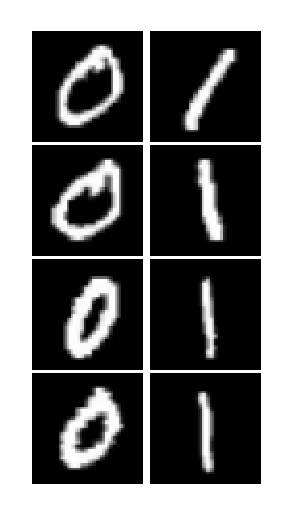
\includegraphics[width=0.045\textwidth]{PaperC/figures/mcts_tikz/vertical_rs/task1_only.eps}};
    \draw[<-] (v43_beg) -- (v3_end);
    
    \node[] (v43_dots) at (13,-7) {\large $\cdots$};
    %\draw[<-] (v4_dots2) -- (v3_beg);
    %\draw[<-] (v4_dots2) -- (v3_mid);
    %\draw[<-] (v4_dots2) -- (v3_end);
    
    \node[squarednode, text=color3] (v43_end) at (14,-7) {\includegraphics[width=0.045\textwidth]{PaperC/figures/mcts_tikz/vertical_rs/task3_only.eps}};
    \draw[<-, purple, very thick] (v43_end) -- (v3_end);
    %\draw[<-] (v4_end) -- (v3_mid);
    %\draw[<-, purple, very thick] (v4_end) -- (v3_end);


    %%% Task 5 level
    \draw[draw=green!50, fill=green!10, very thick, rounded corners] (0,-8) rectangle (16,-10);
    \node[squarednode] (dataset5) at (1.,-9) { \textbf{Task 5} \\ 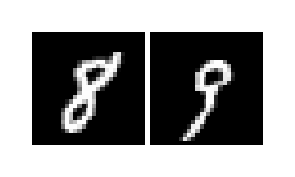
\includegraphics[width=0.08\textwidth]{PaperC/figures/mcts_tikz/dataset_two_images/dataset5.eps}};
    
    \node[squarednode, text=color3] (v51_beg) at (3,-9) {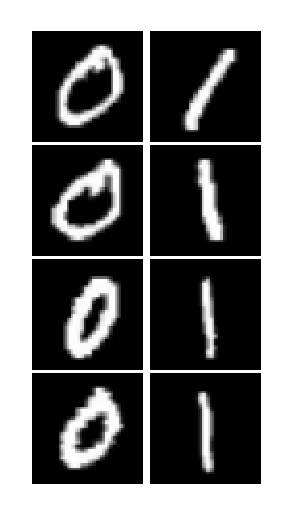
\includegraphics[width=0.045\textwidth]{PaperC/figures/mcts_tikz/vertical_rs/task1_only.eps}};
    \draw[<-, blue, very thick] (v51_beg) -- (v41_beg);
    %\draw[<-] (v5_beg) -- (v4_dots1);
    %\draw[<-] (v5_beg) -- (v4_mid);
    %\draw[<-] (v5_beg) -- (v4_dots2);
    %\draw[<-] (v5_beg) -- (v4_end);
    
    \node[] (v51_dots) at (4,-9) {\large $\cdots$};
    %\draw[<-] (v5_dots1) -- (v4_beg1);
    %\draw[<-] (v5_dots1) -- (v4_dots1);
    %\draw[<-] (v5_dots1) -- (v4_mid);
    %\draw[<-] (v5_dots1) -- (v4_dots2);
    %\draw[<-] (v5_dots1) -- (v4_end);
    
    \node[squarednode, text=color3] (v51_end) at (5,-9) {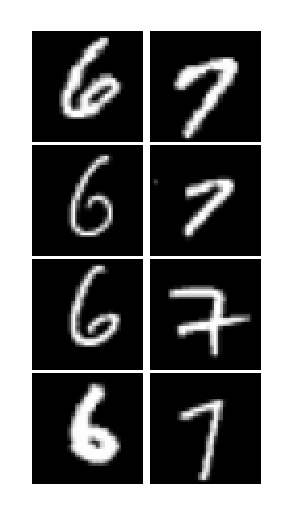
\includegraphics[width=0.045\textwidth]{PaperC/figures/mcts_tikz/vertical_rs/task4_only.eps}};
    \draw[<-] (v51_end) -- (v41_beg);
    
    %\node[squarednode, text=color3] (v52_beg) at (5,-9) {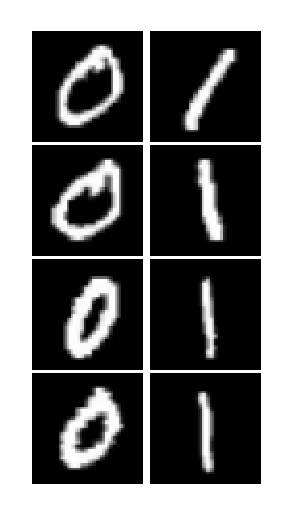
\includegraphics[width=0.045\textwidth]{PaperC/figures/mcts_tikz/vertical_rs/task1_only.eps}};
    
    %\node[squarednode, text=color3] (v5_mid_low) at (6,-9) {\includegraphics[width=0.06\textwidth]{PaperC/figures/mcts_tikz/replay_batches/task5_middle0.eps}};
    %\draw[<-] (v5_mid_low) -- (v4_beg);
    %\draw[<-] (v5_mid_low) -- (v4_dots1);
    %\draw[<-] (v5_mid_low) -- (v4_mid);
    %\draw[<-] (v5_mid_low) -- (v4_dots2);
    %\draw[<-] (v5_mid_low) -- (v4_end);
    
    \node[] (v52_dots) at (6,-9) {\large $\cdots$};
    \draw[<-, dashed] (v52_dots) -- (v41_end);
    
    \node[] (v53_dots) at (7.1,-9) {\large $\cdots$};
    \draw[<-, dashed] (v53_dots) -- (v42_beg);
    
     \node[] (v54_dots) at (8,-9) {\large $\cdots$};
    %\draw[<-] (v5_dots2) -- (v4_beg);
    %\draw[<-] (v5_dots2) -- (v4_dots1);
    %\draw[<-] (v5_dots2) -- (v4_mid);
    %\draw[<-] (v5_dots2) -- (v4_dots2);
    %\draw[<-] (v5_dots2) -- (v4_end);
    
    \node[squarednode, text=color3] (v52_mid) at (9,-9) {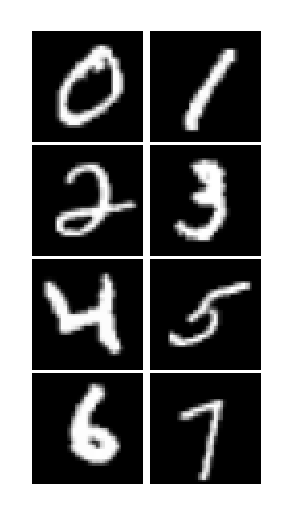
\includegraphics[width=0.045\textwidth]{PaperC/figures/mcts_tikz/vertical_rs/equal_task5.eps}};
    \draw[<-, red, very thick] (v52_mid) -- (v42_mid);
    %\draw[<-] (v5_mid) -- (v4_beg);
    %\draw[<-] (v5_mid) -- (v4_dots1);
    %\draw[<-, red, very thick] (v5_mid) -- (v4_mid);
    %\draw[<-] (v5_mid) -- (v4_dots2);
    %\draw[<-] (v5_mid) -- (v4_end);
    
    \node[] (v55_dots) at (10,-9) {\large $\cdots$};
    
    \node[] (v56_dots) at (11,-9) {\large $\cdots$};
    \draw[<-, dashed] (v56_dots) -- (v42_end);
    
    \node[] (v57_dots) at (12.1,-9) {\large $\cdots$};
    \draw[<-, dashed] (v57_dots) -- (v43_beg);
    %\draw[<-] (v5_dots3) -- (v4_beg);
    %\draw[<-] (v5_dots3) -- (v4_dots1);
    %\draw[<-] (v5_dots3) -- (v4_mid);
    %\draw[<-] (v5_dots3) -- (v4_dots2);
    %\draw[<-] (v5_dots3) -- (v4_end);
    
    %\node[squarednode, text=color3] (v5_mid_high) at (12,-9) {\includegraphics[width=0.06\textwidth]{PaperC/figures/mcts_tikz/replay_batches/task5_middle1.eps}};
    %\draw[<-] (v5_mid_high) -- (v4_beg);
    %\draw[<-] (v5_mid_high) -- (v4_dots1);
    %\draw[<-] (v5_mid_high) -- (v4_mid);
    %\draw[<-] (v5_mid_high) -- (v4_dots2);
    %\draw[<-] (v5_mid_high) -- (v4_end);
    
    \node[squarednode, text=color3] (v53_beg) at (13,-9) {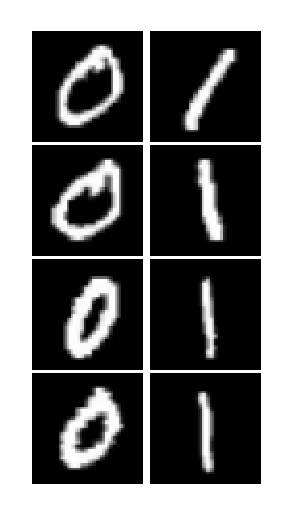
\includegraphics[width=0.045\textwidth]{PaperC/figures/mcts_tikz/vertical_rs/task1_only.eps}};
    \draw[<-] (v53_beg) -- (v43_end);
    
    \node[black] (v58_dots) at (14,-9) {\large $\cdots$};
    
    %\draw[--, dashed] (v5_dots4) -- (v43_dots);
    %\draw[<-] (v5_dots4) -- (v4_mid);
    %\draw[<-] (v5_dots4) -- (v4_dots2);
    %\draw[<-] (v5_dots4) -- (v4_end);
    
    \node[squarednode, text=color3] (v53_end) at (15,-9) {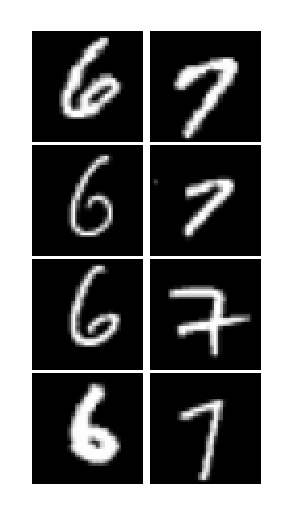
\includegraphics[width=0.045\textwidth]{PaperC/figures/mcts_tikz/vertical_rs/task4_only.eps}};
    \draw[<-, purple, very thick] (v53_end) -- (v43_end);
    %\draw[<-] (v5_end) -- (v4_beg);
    %\draw[<-] (v5_end) -- (v4_dots1);
    %\draw[<-] (v5_end) -- (v4_mid);
    %\draw[<-] (v5_end) -- (v4_dots2);
    %\draw[<-, purple, very thick] (v5_end) -- (v4_end);
\end{tikzpicture}
}
  % \tikzexternalenable
  % \vspace{-15pt}
  % \includegraphics[width=0.95\linewidth]{pixeldag.png}
  % \vspace{-15pt}

	\vspace{-5mm}
    \caption{Tree-shaped action space of possible replay memories of size $M=8$ at every task for Split MNIST.
	%\caption{Tree-shaped action space of possible replay memory compositions with size $M=8$ at every task from the discretization method described in Section \ref{sec:replay_scheduling_in_continual_learning} for Split MNIST. A replay schedule is represented as a path traversal of different replay memory compositions from task 1 to task 5. 
	}
	\vspace{-3mm}
	\label{fig:replay_scheduling_mcts_tree_example}
\end{wrapfigure}
Figure \ref{fig:replay_scheduling_mcts_tree_example} shows an example of a replay schedule tree with Split MNIST~\citeC{C:zenke2017continual} 
where the memory size is $M=8$. Each level corresponds to a task to learn and we show some examples of possible replay memories in the tree that can be evaluated at each task. A replay schedule is represented as a path traversal of different replay memory compositions from task 1 to task 5. At task 1, the memory $\gM_1 = \emptyset$ is empty, while $\gM_2$ is filled with samples from task 1 at task 2. The memory $\gM_3$ can be composed with samples from either task 1 or 2, or equally fill $\gM_3$ with samples from both tasks. All possible paths in the tree are valid replay schedules. We show three examples of possible schedules in Figure \ref{fig:replay_scheduling_mcts_tree_example} for illustration: the \textcolor{blue}{blue} path represents a replay schedule where only task 1 samples are replayed. The \textcolor{red}{red} path represents using memories with equally distributed tasks, and the \textcolor{purple}{purple} path represents a schedule where the memory is only filled with samples from the most previous task.



